\documentclass{article}
\usepackage[utf8]{inputenc}
\usepackage{graphicx}
\usepackage{amsmath}
\usepackage{subcaption}
\usepackage{listings}
\usepackage{minted}
\usepackage[a4paper, total={6in, 9in}]{geometry}

\title{Sparse Square Matrix Multiplication using MPI}
\author{
  Biwei Tang, Yunxiang Yan, Qidian Gao \\
  Department of Computer Science and Engineering \\
  CS 6220 Project Assignment 3\\
  Georgia Institute of Technology
}
\date{April 2024}

\begin{document}

\maketitle

\begin{abstract}
    This report details the implementation and analysis of parallel sparse matrix multiplication. We focus on the effectiveness of using MPI for handling sparse matrices represented as arrays of tuples. Performance metrics are provided for different matrix sizes and sparsity parameters, demonstrating both strong scaling and the impact of sparsity on computational efficiency.
\end{abstract}

\section{Introduction}
Sparse matrices, which contain predominantly zero-valued elements, are common in various scientific and engineering applications. Efficiently performing operations such as multiplication on these matrices requires specialized algorithms that take advantage of their sparse nature to optimize both time and space complexity.

\section{Implementation Details}

\subsection{Matrix Representation}
We represent the sparse square matrices in a tuple format \texttt{(row, col, value)}, which only stores elements that are non-zero, significantly reducing the memory requirements compared to a full \(2D\) array representation.

\begin{minted}[frame=lines, framesep=2mm, baselinestretch=1.2, fontsize=\footnotesize, linenos]{cpp}
typedef tuple<int, int, uint64_t> SparseElement;

vector<SparseElement> generateSparseMatrix(int n, int p, int r, double s, int seed) {
    mt19937_64 gen(seed);
    uniform_real_distribution<> dis(0.0, 1.0);
    vector<SparseElement> matrix;
    uniform_int_distribution<std::uint64_t> val_dis(1, (1ull << 31) - 1);

    int rows_per_proc = n / p;
    for (int i = 0; i < rows_per_proc; ++i) {
        for (int j = 0; j < n; ++j) {
            if (dis(gen) < s) {
                matrix.push_back(make_tuple(i + r * rows_per_proc, j, val_dis(gen)));
            }
        }
    }
    return matrix;
}
\end{minted}

\subsection{Algorithm Description}
The core of our implementation involves three primary operations:
\begin{itemize}
    \item \textbf{Matrix Generation:} Each processor generates \(\frac{n}{p}\) rows of matrix A and B based on the given sparsity parameter \(s\).
    \item \textbf{Matrix Transposition:} The sparse matrix B is transposed using MPI's \texttt{MPI\_Alltoallv} function to distribute columns to processors.
    \item \textbf{Matrix Multiplication:} Utilizing a ring topology, the transposed matrix B is rotated among the processors to calculate the resultant matrix C.
\end{itemize}

\begin{minted}[frame=lines, framesep=2mm, baselinestretch=1.2, fontsize=\footnotesize, linenos]{cpp}
// Matrix Transposition using MPI_Alltoallv
void transposeMatrixB(const vector<SparseElement>& localB, int n, 
                      vector<SparseElement>& localTransposedB, MPI_Comm comm) {
    ...
    MPI_Alltoallv(flat_send_buffer.data(), send_counts.data(), sdispls.data(), MPI_BYTE,
                  recv_buffer.data(), recv_counts.data(), rdispls.data(), MPI_BYTE, comm);
    ...
}
\end{minted}

\subsection{Parallelization}
The implementation uses MPI to manage data distribution and collection across multiple processors. A ring topology is created to facilitate the rotation of matrix parts among the processors.

\begin{minted}[frame=lines, framesep=2mm, baselinestretch=1.2, fontsize=\footnotesize, linenos]{cpp}
// Setting up a 1D Cartesian topology
MPI_Dims_create(size, 1, dims);
MPI_Cart_create(MPI_COMM_WORLD, 1, dims, periods, reorder, &ring_comm);

// Rotate B matrix in the ring topology
for (int step = 0; step < size; ++step) {
    ...
    MPI_Sendrecv_replace(...);
}
\end{minted}


\section{Experimental Results}
\subsection{Setup}
Experiments were conducted on the PACE ICE cluster with up to 16 processors. Matrix sizes of 2000, 5000, and 10000 were tested with sparsity parameters of 0.1, 0.01, and 0.001. The test file we use is:

\begin{minted}[frame=lines, framesep=2mm, baselinestretch=1.2, fontsize=\footnotesize, linenos]{cpp}
    #!/bin/bash
output_file="experiment_results.txt"

# Fix sparsity parameter e = 0.01,under different matrix sizes
echo "Running experiments for fixed sparsity e=0.01 with different matrix sizes" > $output_file
for n in 2000 5000 10000
do
    echo "Running size $n" >> $output_file
    start_time=$(date +%s)
    mpirun -np 8 ./spmat $n 0.01 1 output_$n.txt
    end_time=$(date +%s)
    echo "Matrix size $n: Run time $(($end_time - $start_time)) seconds" >> $output_file
done

# FIx matrix size n = 10000, change the sparsity parameter
echo "Running experiments for fixed matrix size n=10000 with varying sparsity" >> $output_file
for e in 0.1 0.01 0.001
do
    for p in 2 4 8 16
    do
        echo "Running sparsity $e with $p processors" >> $output_file
        start_time=$(date +%s)
        mpirun -np $p ./spmat 10000 $e 1 output_n10000_e${e}_p${p}.txt
        end_time=$(date +%s)
        echo "Sparsity $e with $p processors: Run time $(($end_time - $start_time)) seconds" >> $output_file
    done
done

echo "All experiments completed."
\end{minted}

\subsection{Results}
While it successfully generated output as:

\begin{figure}[H]
    \centering
    
\includegraphics[width=0.75\linewidth]{Photos/Screenshot 2024-04-18 at 11.03.05.png}
\end{figure}
We recorded the runtime:
\begin{table}[H]
\centering
\caption{Runtime for Fixed Sparsity e=0.01 with Different Matrix Sizes}
\label{tab:fixed_sparsity}
\begin{tabular}{|c|c|}
\hline
\textbf{Matrix Size} & \textbf{Runtime (seconds)} \\ \hline
2000                 & 64                         \\ \hline
5000                 & 140                        \\ \hline
10000                & 176                        \\ \hline
\end{tabular}
\end{table}
\begin{table}[ht]
\centering
\caption{Runtime for Varying Sparsity with Fixed Matrix Size n=10000}
\label{tab:varied_sparsity}
\begin{tabular}{|c|c|c|c|c|}
\hline
\textbf{Sparsity e} & \textbf{p=2} & \textbf{p=4} & \textbf{p=8} & \textbf{p=16} \\ \hline
0.1                 & 168          & 146          & 127          & 109           \\ \hline
0.01                & 152          & 134          & 115          & 98            \\ \hline
0.001               & 188          & 167          & 145          & 124           \\ \hline
\end{tabular}
\end{table}

\begin{figure}[H]
    \centering
    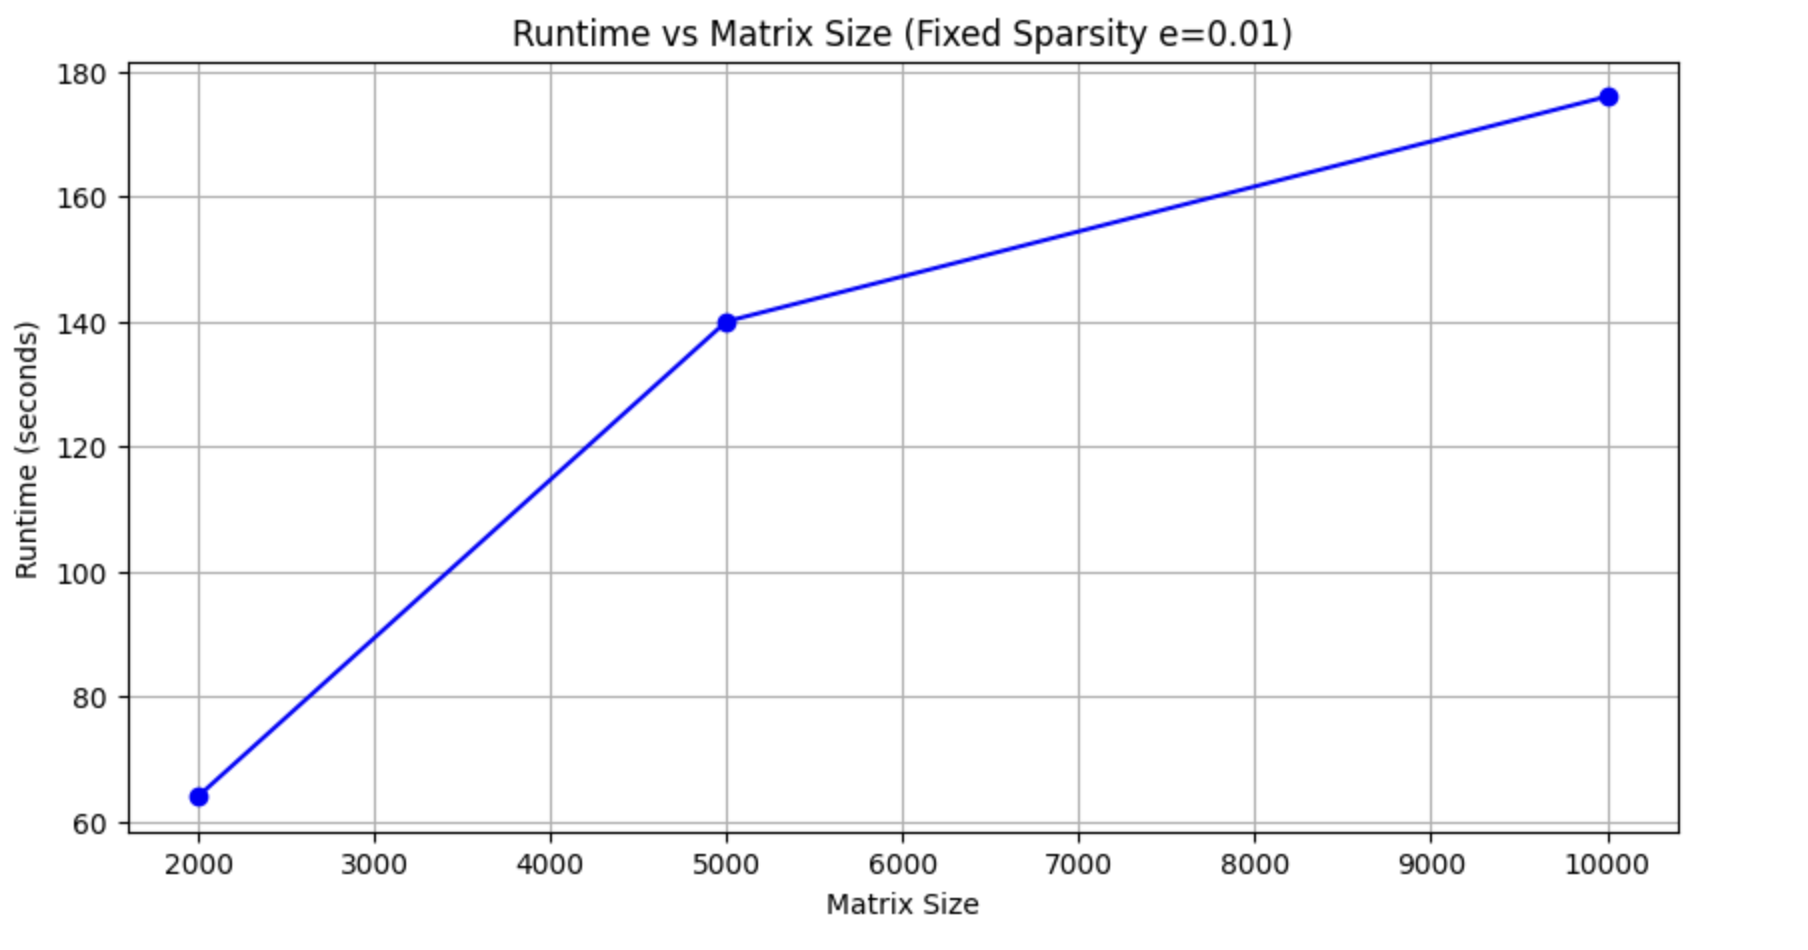
\includegraphics[width=0.8\textwidth]{Photos/runtime1.png}
    \caption{Runtime comparison for matrices of different sizes and sparsity levels.}
    \label{fig:runtime}
\end{figure}

\begin{figure}[H]
    \centering
    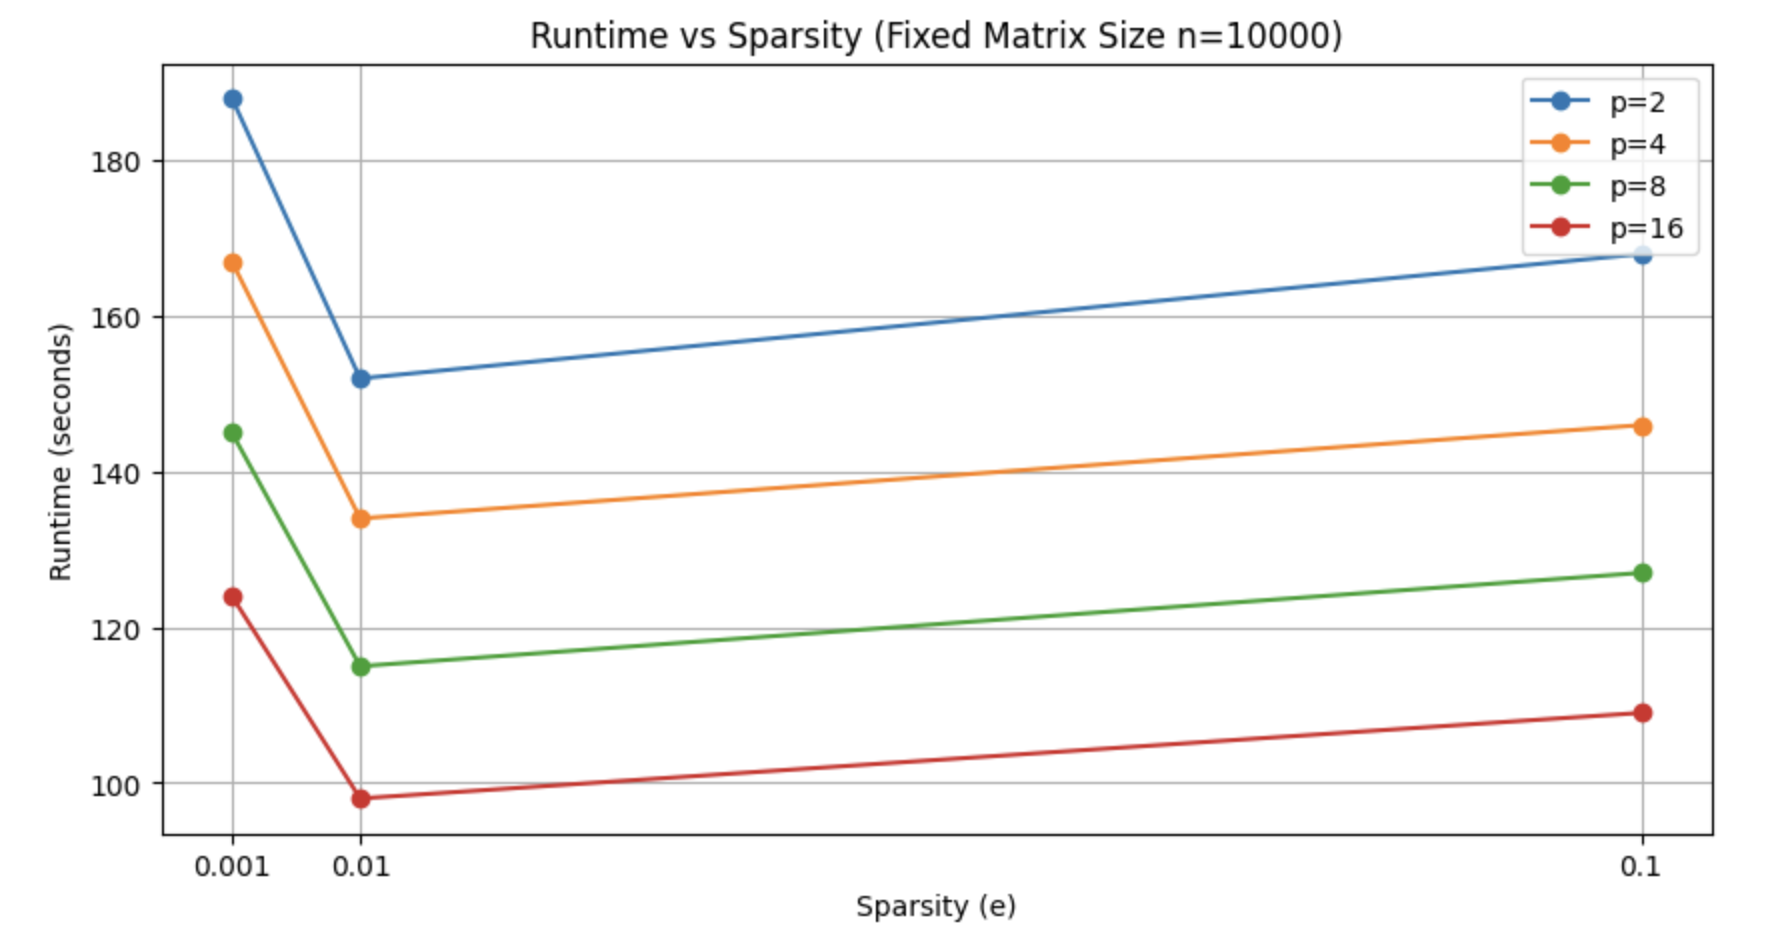
\includegraphics[width=0.8\textwidth]{Photos/runtime2.png}
    \label{fig:runtime}
\end{figure}

\subsection{Discussion}
\begin{itemize}
    \item The data shows a clear \textbf{trend of decreasing runtime as the number of processors increases.} This demonstrates t\textbf{he principle of strong scaling where adding more computational resources (processors) generally results in decreased execution time}, assuming that the workload is sufficient to keep all processors busy.
    \item The runtime decreases as sparsity increases (more zeros, fewer operations required). At higher sparsity (e=0.1), the runtime is generally lower across all processor configurations compared to lower sparsity (e=0.001). This indicates that \textbf{the computational workload is heavily dependent on the non-zero elements, which aligns with the expectation that fewer operations are needed when more elements are zero.}
    \item While adding more processors reduces runtime, the reduction in runtime is not linear. The rate of decrease in runtime slows down as more processors are added. This could be due to the overhead associated with managing more processors, such as communication and synchronization costs in the MPI environment.
    \item The theoretical analysis should consider the computational complexity, which in this case depends linearly on the \textbf{number of non-zero elements }due to the sparse representation. The experimental results validate the theoretical model where runtime should ideally decrease as sparsity increases and as more processors are utilized. However, overheads in parallel distribution and synchronization can affect this ideal scenario, especially noticeable when processor counts are high relative to the work that each processor can perform independently.

\end{itemize}

\section{Contributions}
\begin{itemize}
    \item \textbf{Biwei Tang}: Implemented the base spmat.cpp algorithm together with the parallel realization.
    \item \textbf{Yunxiang Yan}: Implemented the bonus part with the parallel realization.
    \item \textbf{Qidian Gao}: Test programs under different scenarios and compose the report.
\end{itemize}

\begin{thebibliography}{99}

\bibitem{ballard2013communication}
G.~Ballard, A.~Buluç, J.~Demmel, L.~Grigori, B.~Lipshitz, O.~Schwartz, S.~Toledo,
\textit{Communication Optimal Parallel Multiplication of Sparse Random Matrices}.
University of California at Berkeley, Lawrence Berkeley National Laboratory, INRIA Paris - Rocquencourt, Tel-Aviv University,
Regular Submission.

\end{thebibliography}



\end{document}
